\documentclass[11pt,a4paper]{article}
\usepackage[margin=21mm]{geometry}
\usepackage{amsmath,amssymb,booktabs,array,tikz,enumitem,hyperref}
\usetikzlibrary{arrows.meta,positioning}
\setlength{\parindent}{0pt}\setlength{\parskip}{6pt}
\newcommand{\question}[2]{\section*{#1: #2}}
\newcommand{\board}[1]{\begin{tikzpicture}[x=0.39cm,y=0.39cm,baseline=-0.5cm]
\draw(0,0)rectangle(3,3);\foreach\i in{1,2}{\draw(\i,0)--(\i,3);\draw(0,\i)--(3,\i);}
\foreach[count=\i from 0]\v in{#1}{\pgfmathtruncatemacro{\c}{mod(\i,3)}\pgfmathtruncatemacro{\r}{floor(\i/3)}\node at(\c+0.5,2.5-\r){\v};}
\end{tikzpicture}}
\newcommand{\blank}{}
\tikzset{box/.style={draw,rounded corners,align=center,inner sep=6pt},arr/.style={->,>=Stealth}}
\begin{document}
\begin{center}{\Large\bfseries Homework Set 3: Games}\\[4pt]English worked answers with hand-copyable diagrams\end{center}
\small Original questions: requirements/Games-HomeWork Set 3.pdf, pp.\ 1--6.\normalsize

\question{Games1 (p.\ 1)}{Chinese chess branching factor}
\textbf{(A) Count each red piece's legal moves.} Use files $x=1,\ldots,9$ from left to right as viewed on the page, and ranks $y=0,\ldots,9$ from bottom to top. The red back rank is $y=0$; red moves toward increasing $y$. ``Left'' and ``right'' below refer to the drawing, not red's traditional file numbers.
\begin{center}\small\begin{tabular}{l|c|p{7.9cm}|r}\toprule
Piece&Position&Legal destination(s) / directional count&Count\\\midrule
Left rook&$(1,0)$&$(1,1),(1,2),(1,3)$&3\\
Right rook&$(9,0)$&$(9,1),(9,2)$&2\\
Left horse&$(2,0)$&$(1,2),(3,2)$&2\\
Right horse&$(8,0)$&$(7,2),(9,2)$&2\\
Left elephant&$(3,0)$&$(1,2),(5,2)$&2\\
Right elephant&$(7,0)$&$(5,2),(9,2)$&2\\
Left advisor&$(4,0)$&$(5,1)$&1\\
Right advisor&$(6,0)$&$(5,1)$&1\\
General&$(5,0)$&$(5,1)$&1\\
Left cannon&$(4,2)$&Left 3, right 3, down 1, up 6&13\\
Right cannon&$(8,2)$&Left 3, right 1, down 1, up 4 noncaptures + 1 capture&10\\
Soldier 1&$(1,4)$&$(1,5)$&1\\
Soldier 2&$(3,3)$&$(3,4)$&1\\
Soldier 3&$(5,3)$&$(5,4)$&1\\
Soldier 4&$(7,3)$&$(7,4)$&1\\
Soldier 5&$(9,3)$&$(9,4)$&1\\\bottomrule\end{tabular}\normalsize\end{center}
The left cannon is on file 4 in this position, not its usual initial file. Its upward destinations are $(4,3),\ldots,(4,8)$. The right cannon can move upward to $(8,3),\ldots,(8,6)$ and can capture the black horse at $(8,9)$ by jumping over the black cannon at $(8,7)$ as its single screen. It cannot land on the screen or jump it for a noncapture.

Both horses have their sideways legs blocked by friendly back-rank pieces, leaving two forward moves each. The elephants' eyes are clear. The five soldiers have not yet crossed the river, so each has only one forward move. The listed moves do not expose the red general to check or leave the generals facing without an intervening piece.
\[
b=3+2+2+2+2+2+1+1+1+13+10+5=\boxed{44}.
\]
Two different pieces moving to the same destination still produce different resulting positions, so each is a distinct move.

\textbf{(B) One-step look-ahead.} Evaluate the 44 successor positions:
\[\boxed{44\text{ heuristic evaluations}}.\]
\textbf{(C) Three-step look-ahead.} With constant branching factor and evaluation only at the search horizon:
\[\boxed{b^3=44^3=85,184\text{ heuristic evaluations}}.\]
If scores are instead computed for every generated non-root node at depths 1--3, the count would be $44+44^2+44^3=87,164$. The usual depth-limited minimax convention evaluates only horizon leaves.

\newpage
\question{Game2 (p.\ 2)}{Finish the two incomplete games}
Use the following cell numbering:
\begin{center}\board{1,2,3,4,5,6,7,8,9}\end{center}
The question allows completion by intuition, so the following are two possible legal continuations, not claims of unique optimal play. In both games, $X$ moves first and players alternate. Each sequence stops when the full board gives a draw.

\textbf{First game.} The supplied prefix is $X2,O5,X3,O1$. Add
\[\boxed{X9,\ O6,\ X4,\ O7,\ X8}.\]
\begin{center}
\board{O,X,X,\blank,O,\blank,\blank,\blank,\blank}$\;\to\;$
\board{O,X,X,\blank,O,\blank,\blank,\blank,X}$\;\to\;$
\board{O,X,X,\blank,O,O,\blank,\blank,X}\\[9pt]
\board{O,X,X,X,O,O,\blank,\blank,X}$\;\to\;$
\board{O,X,X,X,O,O,O,\blank,X}$\;\to\;$
\board{O,X,X,X,O,O,O,X,X}
\end{center}
$X9$ threatens the right column, which $O6$ blocks. $X4$ blocks $O$'s middle-row threat. $O7$ then creates no unavoidable immediate win, and $X8$ fills the last cell. Neither player has three in a row: \textbf{draw}.

\textbf{Second game.} The supplied prefix is $X2,O3$. Add
\[\boxed{X5,\ O8,\ X1,\ O9,\ X6,\ O4,\ X7}.\]
\begin{center}
\board{\blank,X,O,\blank,\blank,\blank,\blank,\blank,\blank}$\;\to\;$
\board{\blank,X,O,\blank,X,\blank,\blank,\blank,\blank}$\;\to\;$
\board{\blank,X,O,\blank,X,\blank,\blank,O,\blank}$\;\to\;$
\board{X,X,O,\blank,X,\blank,\blank,O,\blank}\\[9pt]
\board{X,X,O,\blank,X,\blank,\blank,O,O}$\;\to\;$
\board{X,X,O,\blank,X,X,\blank,O,O}$\;\to\;$
\board{X,X,O,O,X,X,\blank,O,O}$\;\to\;$
\board{X,X,O,O,X,X,X,O,O}
\end{center}
$O8$ blocks the middle column; $O9$ blocks the main diagonal. $X6$ blocks the right column; $O4$ blocks the middle row. $X7$ blocks $O$'s bottom row and completes a \textbf{draw}.

\newpage
\question{Game3 (p.\ 3)}{Bottom-up value backup}
Use $U=+1$ for an $X$ win, $U=-1$ for an $O$ win, and $U=0$ for a draw. At an $X$-to-move node use MAX; at an $O$-to-move node use MIN:
\[
V(s)=\begin{cases}U(s),&s\text{ terminal},\\
\max_{s'\in\mathrm{children}(s)}V(s'),&X\text{ to move},\\
\min_{s'\in\mathrm{children}(s)}V(s'),&O\text{ to move}.
\end{cases}
\]
\textbf{First label the terminal boards.} In the upper part of the supplied graph, the first two terminal boards are $X$ wins:
\begin{center}
\board{X,O,X,\blank,O,X,O,\blank,X}\quad$+1$\qquad
\board{X,\blank,X,O,O,X,O,\blank,X}\quad$+1$.
\end{center}
The longer upper fork ends in a draw or an $X$ win:
\begin{center}
\board{X,X,O,O,O,X,X,O,X}\quad$0$\qquad
\board{X,O,O,O,O,X,X,X,X}\quad$+1$.
\end{center}
The $O$-to-move node immediately before this fork therefore has $\min(0,1)=0$. Values on a chain with only one pictured successor remain unchanged. Combining this draw branch with the neighboring winning branch gives $\min(1,0)=0$ for the upper $O$-choice, and then the corner-opening/center-response branch has value $\min(1,0)=0$.

The shared middle/lower subgraph also contains a final fork with terminal boards
\begin{center}
\board{O,X,X,X,X,O,O,O,X}\quad$0$\qquad
\board{O,X,X,X,X,O,O,X,O}\quad$+1$.
\end{center}
Again $\min(0,1)=0$. Its alternative branches end in an $X$ win, so the shared subgraph backs up to $0$ when $O$ can select the draw continuation.

\textbf{Back up the opening choices.} The upper branch with first $X$ in the top-left corner has the following values for the three pictured $O$ replies:
\[
O\text{ in center}:0,\qquad O\text{ in top-right corner}:1,
\qquad O\text{ on top edge}:1.
\]
The dashed ``draw possible'' link is an alternative $X$ response in the top-right-corner branch, represented by a symmetric board in the shared subgraph. At that MAX choice, the pictured winning continuation is preferred to the draw: $\max(1,0)=1$.

For first $X$ in the center, the two pictured $O$ replies have values $0$ (top-left corner) and $1$ (top-middle edge). Hence
\[
V(\text{corner first})=\min(0,1,1)=0,\quad
V(\text{center first})=\min(0,1)=0,
\quad V(\text{root})=\max(0,0)=\boxed{0}.
\]

\newpage
\section*{Game3: compact backup diagram}
The diagram compresses single-successor chains and the deeper forks evaluated on the previous page. Labels describe the opening and the opponent's first response.
\begin{center}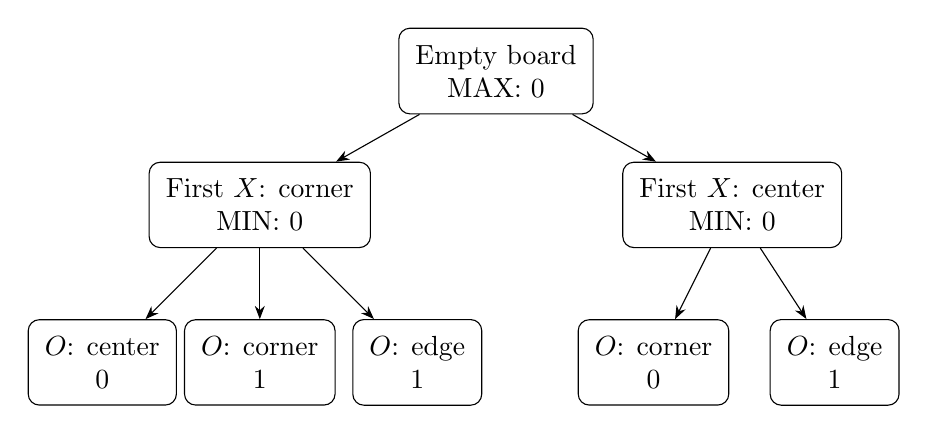
\begin{tikzpicture}[x=1cm,y=1cm]
\node[box](root)at(0,0){Empty board\\MAX: $0$};
\node[box](corner)at(-3,-1.7){First $X$: corner\\MIN: $0$};
\node[box](center)at(3,-1.7){First $X$: center\\MIN: $0$};
\node[box](c1)at(-5,-3.7){$O$: center\\$0$};
\node[box](c2)at(-3,-3.7){$O$: corner\\$1$};
\node[box](c3)at(-1,-3.7){$O$: edge\\$1$};
\node[box](m1)at(2,-3.7){$O$: corner\\$0$};
\node[box](m2)at(4.3,-3.7){$O$: edge\\$1$};
\foreach\a/\b in{root/corner,root/center,corner/c1,corner/c2,corner/c3,center/m1,center/m2}\draw[arr](\a)--(\b);
\end{tikzpicture}\end{center}
\textbf{Answer.} The two opening moves shown in the graph tie with backed-up value $0$. I would put the first $X$ in the \textbf{center}, but the top-left corner is equally good by the supplied minimax values. The center participates in four possible winning lines and is a reasonable preference when a tie must be broken.

This is a backup of the \emph{pictured partial graph}, not a proof that every position labelled $+1$ in it is a forced win in the full game. Omitted replies can change local values. In the complete legal game, perfect play from the empty board gives a draw for center, corner, and edge openings. The graph's displayed values must therefore be interpreted within its displayed choices.

\newpage
\question{Game4 (p.\ 4)}{Two-step look-ahead with a heuristic}
The initial board has $O$ at top-middle and $X$ at center:
\begin{center}\board{\blank,O,\blank,\blank,X,\blank,\blank,\blank,\blank}\end{center}
Let the heuristic be the number of winning lines still open to $X$ minus the number still open to $O$. Back up each two-ply branch using MIN over $O$'s responses. The pictured child scores give:
\begin{center}\begin{tabular}{l|l|c}\toprule
$X$'s candidate move&Scores after $O$'s responses&MIN value\\\midrule
Top-left corner&$2,1,3,1,2,1$&1\\
Middle-left edge&$1,0,2,0,1,1$&0\\
Bottom-left corner&$2,2,3,1,2,2$&1\\
Bottom-middle edge&$1,1,0$ (symmetry representatives)&0\\\bottomrule\end{tabular}\end{center}
At the root, $X$ chooses MAX:
\[\max(1,0,1,0)=\boxed{1}.\]
\textbf{The best pictured moves are the top-left and bottom-left corners.} By left-right symmetry, the corresponding right-hand corners tie as well.

Among the two pictured best moves, I prefer the \textbf{bottom-left corner}. Its response scores are $2,2,3,1,2,2$, whereas the top-left scores are $2,1,3,1,2,1$. Both have the same worst-case score of 1, but the bottom-left move gives more favorable scores against most other replies. This is a secondary preference, not a higher minimax value or a guaranteed win.

\begin{center}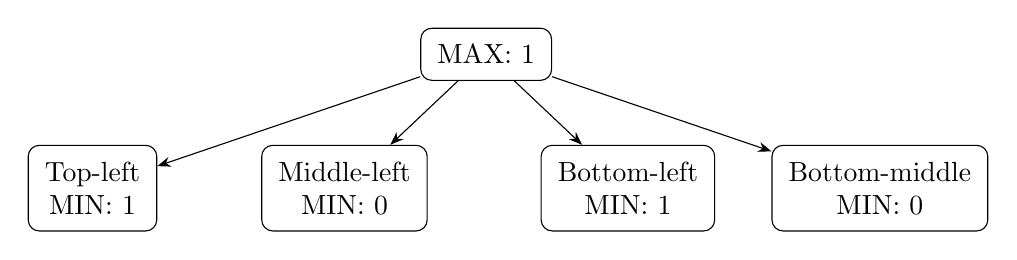
\begin{tikzpicture}[x=1cm,y=1cm]
\node[box](root)at(0,0){MAX: $1$};
\node[box](a)at(-5,-1.7){Top-left\\MIN: $1$};\node[box](b)at(-1.8,-1.7){Middle-left\\MIN: $0$};
\node[box](c)at(1.8,-1.7){Bottom-left\\MIN: $1$};\node[box](d)at(5,-1.7){Bottom-middle\\MIN: $0$};
\foreach\n in{a,b,c,d}\draw[arr](root)--(\n);
\end{tikzpicture}\end{center}
After the preferred move, the board is
\begin{center}\board{\blank,O,\blank,\blank,X,\blank,X,\blank,\blank}\end{center}

\newpage
\question{Game5 (pp.\ 5--6)}{Properties of the complete search tree}
Use the empty board as depth 0, let $X$ move first, and stop expanding a node immediately after a win or when the board is full. A leaf counts a complete \emph{move history}, not a symmetry class or a distinct final board.

\textbf{1. Why do leaves occur at depths 5,6,7,8,9?}
A player needs three marks to win. $X$ places its third mark at move 5, so no win is possible earlier. $O$ can first win at move 6. Further wins can occur at moves 7,8,9; any full board at move 9 is terminal even without a win. Thus the possible terminal depths are exactly 5 through 9.

\textbf{2. Why is every depth-5 leaf worth $+1$?}
At depth 5, $X$ has three marks and $O$ has two. The board is not full and $O$ cannot yet have a line. A terminal board at this depth must therefore be an $X$ win, with utility $+1$.

\textbf{3. Why is every depth-6 leaf worth $-1$?}
The sixth move belongs to $O$. Any $X$ win would have occurred on move 5 and would already have stopped the game. Therefore a new leaf at depth 6 is an $O$ win, with utility $-1$.

\textbf{4. Why do depth-9 leaves have values $0$ or $+1$?}
The ninth move belongs to $X$. If it creates a line, $X$ wins and the utility is $+1$; otherwise the full board is a draw with utility 0. $O$ cannot newly win on $X$'s move, and any earlier $O$ win would already have ended the game.

\textbf{5. Number of depth-5 leaves.}
There are eight possible winning lines for $X$. For a chosen line, its three marks can be placed in $3!$ orders. $O$ chooses two of the other six cells and can place them in $2!$ orders. No earlier win is possible, and three $X$ marks cannot form two distinct lines. Therefore
\[
N_5=8\times3!\times\binom62\times2!
=8\times6\times15\times2=\boxed{1,440}.
\]

\textbf{6. Number of depth-6 leaves (optional).}
Choose $O$'s winning line, arrange its three moves, and choose and arrange $X$'s three other cells:
\[
8\times3!\times\binom63\times3!=5,760.
\]
Exclude histories in which $X$ already won on move 5. There are 12 ordered pairs of disjoint winning lines: choose $O$'s row and a different row for $X$ ($3\times2$), or choose $O$'s column and a different column ($3\times2$). Every diagonal intersects every other winning line. Each pair allows $3!3!=36$ move orders. Hence
\[
N_6=5,760-12\times36=\boxed{5,328}.
\]

\newpage
\section*{Game5: depth-9 counting (optional)}
\textbf{7. Number of depth-9 leaves.} Count legal move histories recursively, stopping immediately at any terminal board. Define $L_d(s,t)$ as the number of terminal continuations of length $d$ from state $s$ with player $t$ to move:
\[
L_0(s,t)=\begin{cases}1,&s\text{ is terminal},\\0,&\text{otherwise},\end{cases}
\]
and for $d>0$,
\[
L_d(s,t)=\begin{cases}
0,&s\text{ is terminal},\\
\displaystyle\sum_{a\in\mathrm{legal}(s,t)}L_{d-1}(\mathrm{Result}(s,a),\bar t),&\text{otherwise}.
\end{cases}
\]
Applying this recurrence to the empty board, without merging repeated boards or symmetric positions, gives
\begin{center}\begin{tabular}{c|r|r|r|r}\toprule
Depth&$X$ wins&$O$ wins&Draws&Terminal histories\\\midrule
5&1,440&0&0&1,440\\
6&0&5,328&0&5,328\\
7&47,952&0&0&47,952\\
8&0&72,576&0&72,576\\
9&81,792&0&46,080&127,872\\\bottomrule\end{tabular}\end{center}
Thus
\[
\boxed{N_9=81,792+46,080=127,872}.
\]
The numbers were obtained by actual exhaustive enumeration and independently checked. The draw count also has a direct check: there are 16 full draw boards, each with five $X$ marks and four $O$ marks. Every order of those marks is legal because no subset of a draw board contains a winning line. Therefore
\[
16\times5!\times4!=46,080.
\]
The total number of terminal histories across all depths is
\[
1,440+5,328+47,952+72,576+127,872=255,168.
\]
Using $9!$ for depth 9 would incorrectly include games that should have stopped at an earlier win. The first-move symmetry reduction suggested by the small sketch must not be used when counting leaves of the complete unmerged tree shown on the next page of the question.
\end{document}
